%!TEX root = Thesis.tex
\chapter{Implementation and Evaluation}
	The chapter contains practical part of the work, describing implementation of modules defined in the Chapter 4 within convincing scenario. The prototype implements major aspects proposed in the concept, including following tiers:
	 \begin{itemize}
		\item \textbf{Client Tier} includes adaptive GUI with related libraries, modules for dynamic content updates and session management;
		\item \textbf{Application Tier} contains XMPP server with protocol extensions, ensuring appropriate interface for collaboration between tiers;
		\item \textbf{Data Tier} contains descriptional metadata of sensors and is responsible for streaming text, images or arbitary data provided by heterogeneous sources.
	\end{itemize}
	To make precise evaluation, system will use real data from temperature sensor which is provided by ACDSense project, together with TU Dresden, BTU Cottbus-Senftenberg and RWTH Aachen University. It is located in the room INF3084, Faculty of Computer Science, Chair of Computer Science.


\section{Development Environment}
 \subsection{Programming language and dependencies}
	In order to maximize application compatibility, standard web-stack tools have been selected for this work: Javascript for frontend logic, HTML\footnote{HTML specification, \url{http://www.w3.org/wiki/HTML/Specifications}} for layout markup, CSS\footnote{CSS specification, \url{http://www.w3.org/Style/CSS/specs.en.html}} for block styling.

	To select additional software tools responsible for css selectors, function chaining, event handlers, AJAX etc, a comprehensive comparison of libraries was made, including most popular web toolkits like jQuery\footnote{jQuery Javascript library, \url{http://jquery.com/}}, Dojo\footnote{Dojo documentation, \url{http://dojotoolkit.org/features/}}, Prototype\footnote{Prototype documentation, \url{http://prototypejs.org/}}, Yahoo User Interface(YUI) and ExtJS\footnote{ExtJS documentation,\url{http://docs.sencha.com/extjs/4.2.2/}}, as shown in the Table 5.1. 
	\begin{table}[H]
	\centering
	\begin{tabular}{|L{3cm}|l|L{2cm}|l|L{2cm}|L{2cm}|}
	\hline
	Target 			& jQuery & Dojo & Prototype & YUI & ExtJS \\
	\hline
	\hline
	License		& MIT & BSD \& AFL & MIT & BSD & GPL and Commercial \\
	\hline
	Size		& 32 kB & 41 kB & 46–278 kB & 31 kB & 84–502 kB \\
	\hline
	Dependencies		& JavaScript & JavaScript + HTML & JavaScript &  Javascript + HTML + CSS & JavaScript \\
	\hline
	Layout Grid		& yes & yes & yes & - & yes  \\
	\hline
	DOM wrapped		& yes & yes & yes & no & yes \\
	\hline
	Data retrieval formats		& XML, HTML & XML, HTML, CSV, ATOM & - & yes & XML  \\
	\hline
	Server push data retrieval		& yes & yes & - & via plugin & yes \\
	\hline 		
	Touch events		& with plugin & yes & yes & - & yes \\
	\hline 
	\end{tabular}
	\caption[Comparison of JavaScript frameworks]{Comparison of JavaScript frameworks}
	\label{tab:JS_frameworks}
	\end{table}
	Also the most important part is browser support which is presented in the Table 5.2 . jQuery\footnote{jQuery browser support, \url{http://jquery.com/browser-support/}}, Dojo\footnote{Dojo browser support,\url{http://livedocs.dojotoolkit.org/releasenotes/1.4}}, Prototype\footnote{Prototype browser support, \url{http://prototypejs.org/doc/latest/Prototype/Browser/index.html}}, YUI\footnote{YUI browser support, \url{http://yuilibrary.com/yui/environments/}}, ExtJS\footnote{ExtJS browser support, \url{http://www.sencha.com/products/extjs/}}.

	\begin{table}[H]
	\centering
	\begin{tabular}{|r|l|l|l|l|l|}
	\hline
	Target 			& jQuery & Dojo & Prototype & YUI & ExtJS \\
	\hline
	\hline
	Chrome		& 1+ & 3 & 1+ & - & 10+ \\
	\hline
	Opera		& 9+ & 10.50+ & 9.25+ & 10.0+ & 11+ \\
	\hline
	Safari		& 3+ & 4 & 2.0.4+ & 4.0 & 4+ \\
	\hline
	Mozilla Firefox		& 2+ & 3+ & 1.5+ & 3+ & 3.6+ \\
	\hline
	Internet Explorer		& 6+ & 6+ & 6+ & 6+ & 6+ \\
	\hline
	\end{tabular}
	\caption[Browser Support]{Browser Support}
	\end{table}


	 Considering aforesaid evaluation, jQuery library has been selected as a main Javascript dependency. The goal of such software components selection is to make resulting code more short, readable, and easier to support for other developers.

    \subsection{XMPP Client on JavaScript}

	Web applications are cross-platform, easily deployable, and come with a large user base already familiar with them. Web technologies rely on HTML, and it is usually the case that tools for manipulating HTML are also compatible with XML, making a good basis for work with XMPP stanzas. In order to implement web-based client-side application supporting XMPP streams Strophe.js\footnote{Strophe.js an XMPP library for JavaScript, MIT licensed, \url{http://strophe.im/strophejs/}} library was used.

    \textbf{Strophe.js} is a library for invoking the XMPP protocol from a web-browser, targeting web clients. While most of XMPP libraries are focused on chat-based applications, Strophe.js can to also power real-time games, notification systems and search engines, etc. It is production-ready since 2009, and therefore well tested, documented, and easy to extend. It uses BOSH, a standard binding of XMPP to HTTP using long polling.

\subsection{Frontent Frameworks}
   \subsubsection{Integrating CSS toolkit}
	Twitter Bootstrap was selected as one of the most popular and widely used css frameworks nowadays, offering basic style and usability components for web pages, such as responsive CSS grid, adaptive class mixins, various widgets, etc. 

	It consists of four main modules:
	\begin{enumerate}
	\item Scaffolding – global styles, responsive 12-column grids and layouts. Has some expressive features like tablets and mobile grids which maintain the grid column structure instead of collapsing the grid columns into individual rows when the viewport is below 768 or 480 pixels wide.
	\item Base CSS – this includes fundamental HTML elements like tables, forms, buttons, and images, styled and enhanced with extensible classes.
	\item Components – collection of reusable components like dropdowns, button groups, navigation controls (tabs, pills, lists, breadcrumbs, pagination), thumbnails, progress bars, media objects, and more.
	\item JavaScript – jQuery plugins which bring the above components to life, and adding transitions, modals, tool tips, popovers, scrollspy, carousel, typeahead, affix navigation, and more. 
	\end{enumerate}

	It was decided to use first three modules for GUI development, maximally reducing Javascript dependencies. All animations, appearence, and dynamic adaptivity was done by using special tags, anchors and classes.

 	Examples of used modules are shown on a screenshots in the section \ref{section:use-case-scenario}. It contains buttons, navigation tabs bar, log in form, search field, 4/3/2-columns  grid layout, modals, tooltips and carousel for previews.

\subsubsection{Integrating JavaScript MVC}
	As mentioned in the section \ref{section:web-frontend}, it is important to implement the system in a loosely-coupled way. Visualization, user management, content retrieving and data aggregation modules have to be separated and accessable through strictly defined interfaces.

	In order to structure the code and enforce module decoupling, AngularJS\footnote{AngularJS,\url{http://angularjs.org/}} framework was selected. It assists running single-page application with a goal to augment it with model–view–controller (MVC) capability, making development, testing and support simpler.

	Angular.js parces HTML that contains additional custom tag attributes; it then obeys the directives in those custom attributes, and binds input or output parts of the page to a model represented by standard JavaScript variables. The values of those JavaScript variables can be manually set, or retrieved from static or dynamic JSON resources\cite{ wiki:angular}. AngularJS is a toolset for building the framework most suited to application development. It is extensible and works well with other libraries such as jQuery. Every feature can be modified or replaced to suit unique development workflow and feature needs.

    The framework adapts and extends traditional HTML to better serve dynamic content through two-way data-binding (Figure \ref{img:data-binding}) that allows automatic synchronization of models and views. As a result, AngularJS deemphasizes DOM manipulation and improves testability.

	    \begin{figure}[!ht]
		\centering
		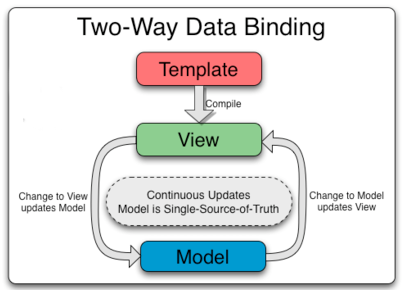
\includegraphics[scale=0.8]{images/2wayBinding.png}   
		\caption[Two-way data binding]{Two-way data binding\footnote{Angular JS Two-Way Data Binding,\url{http://docs.angularjs.org/guide/databinding}}}
		\label{img:data-binding}
		\end{figure}

	\emph{Design goals}
	\newline
	Decouple DOM manipulation from application logic. This improves the testability of the code. Decouple the client side of an application from the server side. This allows development work to progress in parallel, and allows for reuse of both sides.	Angular follows the MVC pattern of software engineering and encourages loose coupling between presentation, data, and logic components. Using dependency injection, Angular brings traditional server-side services, such as view-dependent controllers, to client-side web applications. Consequently, much of the overheads on the backend is reduced, leading to much lighter web applications.

   \emph{Two-way data binding}
   \newline
	AngularJS two-way data binding is a most notable feature and reduces the amount of code written by relieving the server backend from templating responsibilities. Instead, templates are rendered in plain HTML according to data contained in a scope defined in the model. The \$scope service in Angular detects changes to the model section and modifies HTML expressions in the view via a controller. Likewise, any alterations to the view are reflected in the model. This circumvents the need to actively manipulate the DOM and encourages bootstrapping and rapid prototyping of web applications.

	The way Angular templates works is different, as illustrated on the Figure \ref{img:tmv}. They are different because first the template (which is the uncompiled HTML along with any additional markup or directives) is compiled on the browser, and second, the compilation step produces a live view. Any changes to the view are immediately reflected in the model, and any changes in the model are propagated to the view. This makes the model always the single source for the application state, simplifying the programming model for the developer. View is therefore an instant projection of a model.

	    \begin{figure}[!ht]
		\centering
		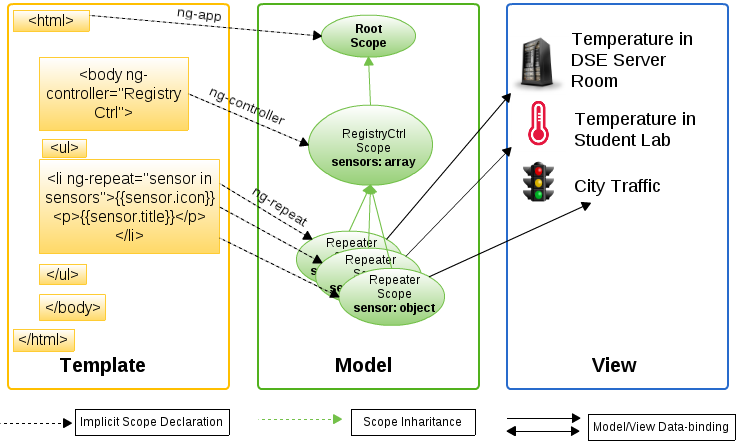
\includegraphics[scale=0.6]{images/3wayBinding.png}   
		\caption[Template Model View]{Template Model View} 
		\label{img:tmv}
		\end{figure}
        
    Because the view is just a projection of the model, the controller is completely separated from the view and unaware of it. As shown on the figure above, the resulting view can be applied to every data available on a backend. Model handler automaticaly generates a view for every new sensor. No need to change code or add new id and dependent handlers, variables, channels. 
    
    The template declaire the structure of what have to be shown on user view. Model repeats to generate the same view of every sensor in the list, which is coming from a controller as parameter {{sensor}} with possible attributes {{sensor.icon}} and {{sensor.titel}}, till the list of registered sensors will be finished.

    The code of such flow is shown on the Listing~\ref{angular_template}
    \begin{lstlisting}[label=angular_template,caption=Template registry.html]
<div id="sensor_list">
    <div class="grid-sizer"></div>
    <div class="masonry-brick sensor-wrapper" id="{{sensor.id}}" ng-repeat="sensor in sensors | filter:{title: query}">
        <div class="sensor" ng-controller="RegistryCtrl" ng-click="open()">
            <div class="icon">
                <img class="img-responsive" ng-src="{{sensor.icon}}">
                <h4>{{sensor.title}}</h4>
                <span class="label label-success" ng-show="user.check_subscribe(sensor.id)">Subscribed</span>
            </div>
            <div ng-show="sensor.picture">
                <img class="img-responsive" ng-src="{{sensor.picture}}">
            </div>
            <span class="description">{{sensor.description}}</span>
        </div>
    </div>
</div>
    \end{lstlisting}

    Model is explicitly integrated to the HTML by using directives: ng-repeat, ng-src, ng-click and sensor prototype attributes {{sensor.*}}, as shown on the listing~\ref{angular_template}. Next, listing~\ref{angular_controller} shows the ``RegistryCtrl'' controller implementation.

    \begin{lstlisting}[label=angular_controller,caption=Controller controller.js]
var sensdash_controllers = angular.module("sensdash.controllers", []);

sensdash_controllers.controller("RegistryCtrl", ["$scope", "Registry", "User",
    function ($scope, Registry, User) {
        Registry.load().then(function(sensors){
            $scope.sensors = sensors;
        });
        $scope.user = User;
    }]);
    \end{lstlisting}

	On the Listing~\ref{angular_service} a Registry service is shown, an application module that asynchronously requests and parses JSON responses from registries, concatenate them and returns single sensors array based on a factory pattern. Such type of loose coupling helps to avoid code overhead and simplify maintenance.  

    \begin{lstlisting}[label=angular_service,caption=Factory Service of Registry]
var sensdash_services = angular.module('sensdash.services', ['ngResource']);

sensdash_services.factory("Registry", ["$http", "$q", "User", function ($http, $q, User) {
    var registry = {
        load: function () {
            var requests = [];
            var all_registries = User.registries.concat(Config.REGISTRIES);
            for (var i = 0; i < all_registries.length; i++) {
                requests.push($http.get(all_registries[i]));
            }
            var q = $q.all(requests);
            var flat_list = q.then(function (result) {
                var list = [];
                for (var i = 0; i < result.length; i++) {
                    list = list.concat(result[i].data);
                }
                return list;
            });
            return flat_list;
        }
    }
    return registry;
}])
    \end{lstlisting}


\section{Interface Implementation}
	 According to the concept architecture, system has to implement two main intefaces:
	 \begin{itemize}
	 \item Registry -- Directory Manager
	 \item Data Hub -- DataStream Manager and AuthHandler 
	 \end{itemize}
	 Implementation of aforesaid interfaces and related modules will be described next.

\subsection{Registry -- Directory Manager}
    A Directory Manager on the Listing~\ref{angular_registry}
    \begin{lstlisting}[label=angular_registry,caption=Factory Service of Registry]
    sensdash_services.factory("Sensor", ["$resource",
    function ($resource) {
        return $resource("api/sensors/:sensorId", {}, {
            query: {method: "GET", params: {sensorId: "all"}, isArray: true}
        });
    }]);
    \end{lstlisting}
It send HTTP GET request to all Registries existed in user.registries[]. Than continues parsing Registries data in JSON format as shown On the Listing~\ref{angular_service}. 

\subsection{Data Hub -- DataStream Manager and AuthHandler}
	A DataStream Manager maintains an XMPP connection and provides access to it via HTTP long polling technique.
	    \begin{figure}[!ht]
		\centering
		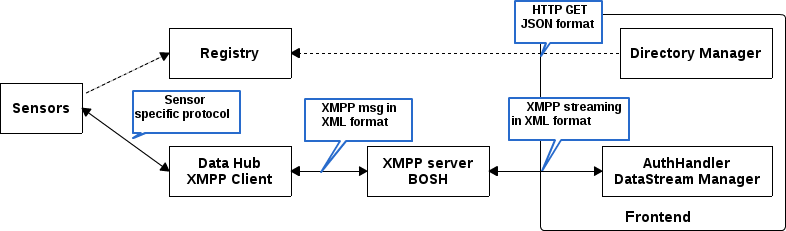
\includegraphics[scale=0.6]{images/XMPPflow.png}   
		\caption[System Interfaces]{System Interfaces}
        \label{img:interface}                      
		\end{figure}

	The browser and the DataStream Manager communicate over HTTP using a Bidirectional-streams Over Synchronous HTTP(BOSH). Essentially, BOSH helps an HTTP client to establish a new XMPP session, then transports stanzas back and forth over HTTP wrapped in a special <body> element. It also provides some security features to make sure that XMPP sessions cannot be easily hijacked. The DataStream Manager communicates with the XMPP server as a normal client. In this way, an HTTP application can control a real XMPP session. Because of the efficiency and low latency afforded by the long polling technique, the end result competes with native connections.

\subsubsection{XMPP Stanzas}
	In XMPP Message transfering is accomplished by the sending and receiving of XMPP stanzas over an XMPP stream. Three basic stanzas make up the core XMPP toolset. These stanzas are <presence>, <message>, and <iq>. Each type of stanza has its place and purpose, and by composing the right kinds of quantities of these stanzas, sophisticated behaviors can be achieved. An XMPP stream is a set of two XML documents, one for each direction of communication. These documents have a root <stream:stream> element. The children of this <stream:stream> element consist of routable stanzas and stream related top-level children. Each stanza is an XML element, including its children. The end points of XMPP communication process input and generate output on a stanza-by-stanza basis. The following example shows a simplified and short XMPP session on the listing~\ref{code:stanzas}
		\begin{lstlisting}[label=code:stanzas,caption=Stanzas Format]
		<stream:stream>
			<iq type="get">
				<query xmlns="jabber:iq:roster"/>
			</iq>
			<presence/>
			<message to="user@inf.tu-dresden.de"
					 from="room@inf.tu-dresden.de/chatroom"
			         type="chat">
			    <body>Room test</body>
			</message> 
			<presence type="unavailable"/>
		</stream:stream>
		\end{lstlisting}

	In this example, sensor created an XMPP stream by sending the opening <stream:stream> tag. With the stream open, it sends a first stanza, an <iq> element. This <iq> element requested sensor roster. Next, it notifies the server that it was online and available with a <presence> stanza. After noticing that user was online, it sent him a short <message> stanza. Finally, sensor sent another <presence> stanza to inform the server she was unavailable and closed the <stream:stream> element, ending the session.
    
    \subsubsection{Server communication}
	The set of XMPP servers that can mutually communicate forms an XMPP network. The set of public XMPP servers forms the global, federated XMPP network. If a server does not speak the server-to-server protocol, it becomes an island, unable to communicate with external servers. An XMPP server will usually allow users to connect to it. It is, however, also possible to write applications or services that speak the server-to-server protocol directly in order to improve efficiency by eliminating routing overhead. Anyone can run an XMPP server, and full-featured servers are available for nearly every platform. Ejabberd, Openfire, and Tigase are three popular open source choices that will work on Windows, Mac OS X, or Linux systems. Several commercial XMPP servers are available as well, including M-Link and Jabber XCP.
	
	\subsubsection{Generic Connections}
	Before any stanzas are sent, an XMPP stream is necessary. Before an XMPP stream can exist, a connection must be made to an XMPP server. XMPP includes some sophisticated support for establishing connections to the right servers. Typically clients and servers utilize the domain name system (DNS) to resolve a server's domain name into an address they can connect to. Email services in particular use mail exchange (MX) records to provide a list of servers that handle mail for a given domain so that one well-known server address does not have to handle every service. Email, being an early Internet application, got special treatment in DNS. These days, service records (SRV) are used to provide a similar function for arbitrary services. The first thing an XMPP client or server does when connecting to another XMPP server is to query the appropriate SRV record at the server’s domain. The response may include multiple SRV records, which can be used to load balance connections across multiple servers. If an appropriate SRV record cannot be found, the application tries to connect to the given domain directly as a fallback. Most libraries also allow you to specify a server to connect explicitly.

	\subsubsection{Web-based Connections}
	XMPP connections are managed through the Connection object, implemented by Strophe library. DataStream Manager includes a pool of BOSH connection managers that require HTTP-bind URL to establish connections. Major XMPP servers come with support for BOSH built in, and they typically expose HTTP-bind service at http://example.com:5280/http-bind or http://example.com:5280/xmpp-httpbind.

	Although getting XMPP into a browser certainly involves extra development effort, this technique has some advantages over direct XMPP connections:
	\begin{itemize}
	\item Interactions with the connection manager are request by request, which allows the client to move from network to network. The managed connection stays available even if the end user's IP address changes several times.
	\item Because one failing request doesn't terminate the managed connection, managed sessions are extremely robust and tolerant of temporary network failure.
	\item Because connection managers cache and resend data for a request, no needs to worry about losing data when connection is interrupted.
	\item HTTP is extremely firewall friendly, and because most connection managers run on standard HTTP ports, managed connections still work even in limited network environments that don’t allow anything but HTTP.
	\end{itemize}

	Creation of the new Strophe.Connection object is shown on listing ~\ref{code:js_object}. Once a connection object was created, calls connect() and disconnect() can be used to start and end communication with the server:

	    \begin{lstlisting}[label=code:js_object,caption=Stanzas Format]
		var conn = new Strophe.Connection("http://example.com:5280/xmpp-httpbind");
		// starting a connection to example.com
		conn.connect(jid, "password", callback);
		// disconnecting
		conn.disconnect();
	    \end{lstlisting}

	The first two parameters to connect() are the JID and password to use to authenticate the session, and the last parameter is the callback function. The callback function will be called with a single parameter that is set to one of the statuses (CONNECTED, DISCONNECTED, AUTHFAIL, CONNFAIL etc.). An example of function that checks login credentials and saves cookies once the connection reaches the CONNECTED phase is shown on listing~\ref{code:connect_callback}: 

	\begin{lstlisting}[label=code:connect_callback,caption=Stanzas Format]
		var update_connection = function (status) {
            ...
		if (status == Strophe.Status.CONNECTED) {
                    console.log('XMPP connection established.');
                    $scope.xmpp.connection.send($pres().tree());
                    // Login was successful, save cookies
                    $scope.process = '';
                    $scope.in_progress = false;
                    $cookies.myID = $scope.user.jid;
                    $cookies.myToken = $scope.user.pass;
                    User.reload();
                }
	\end{lstlisting}

Every time the connection changes its status, this callback function is executed. The callback function simply ignores any status but the CONNECTED status, and disconnects once the connection has reached that status.

\subsubsection{Session Mechanism}
XMPP is a TCP-based protocol, like HTTP, and communication happens over an established, mostly reliable socket between two endpoints. The BOSH extension to XMPP provides a bridge between this bidirectional, stateful protocol and HTTP, which is unidirectional and stateless. Because a web browser cannot directly connect to an XMPP server, a BOSH connection manager responds to requests from a browser using HTTP and uses them to manage an XMPP connection on behalf of the user (Figure~\ref{img:xmpp-bosh}).  XMPP's basic model of communication is Client -> Server -> Server -> Client, and in support of this it defines a Client to Server protocol and a Server to Server protocol.
  \begin{figure}[!ht]
  \centering
  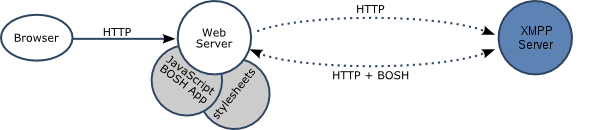
\includegraphics[scale=0.6]{images/xmpp-bosh.png}   
  \caption[BOSH]{XMPP BOSH}
  \label{img:xmpp-bosh}                        
  \end{figure} 

Aside from the socket needed for XMPP communication, each managed connection has two other pieces of data associated with it: the session identifier(SID) and the request identifier(RID). SID stands for Session Identifier. This uniquely identifies the managed XMPP connection, and it is often a long, opaque alphanumeric string. Even though it is enough to identify the session, it is not very useful on its own. The RID identifies a particular HTTP request associated with a BOSH-managed connection. Before a connection is established, the client sends a random RID to the DataStream Manager along with its first request. Each subsequent request increments the RID by one. The SID and the RID together provide enough information to interact with the underlying XMPP connection. Because the RID is generated randomly from a very large range of numbers, it is virtually impossible to guess the RID. Also, the DataStream Manager will reject RIDs that fall outside of a narrow window around the current request. In this way, the BOSH-managed connection is tolerant of small errors like out of order delivery but robust to attacks like hijacking the connection. Because these two identifiers are enough to both address and make use of a managed XMPP session, if an application knows the SID and the RID, it can take over or attach to the underlying session.

The attach() function demonstrats sending SID and RID through a BOSH connection in the Listing~\ref{BOSH_callback}):
	    \begin{lstlisting}[label=BOSH_callback,caption=BOSH Callback]
		var connection = new Strophe.Connection(BOSH_URL);
        connection.attach(jid, sid, rid, callback);
	    \end{lstlisting}

BOSH sessions can be encrypted, and often the underlying XMPP sessions are encrypted as well. Because XMPP makes use of SASL, the authentication mechanisms are strong.

\subsection{XEP-0045: Multi-User Chat}
Traditionally, instant messaging is thought to consist of one-to-one chat rather than many-to-many chat, which is called variously ``groupchat'' or ``text conferencing''. The Jabber/XMPP community developed and implemented a basic groupchat protocol since 1999. That ``groupchat 1.0'' protocol provided a minimal feature set for chat rooms but was rather limited in scope. The Multi-User Chat or MUC builds on the older groupchat 1.0 protocol in a backwards-compatible manner but provides advanced features such as invitations, message presence, room moderation and administration, and specialized room types\footnote{XEP0045, \url{http://xmpp.org/extensions/xep-0045.html}}.

\subsubsection{Requirements}
In scope of this Master Thesis only the limited functionality is required, provided by Jabber-based multi-user chat services. 

Each room is identified as a ``room JID'' <room@service> (e.g. <jdev@conference.jabber.org>), where ``room'' is the name of the room and ``service'' is the hostname at which the multi-user chat service is running. Each occupant in a room is identified by ``occupant JID'' <room@service/nick>, where ``nick'' is the room nickname of the occupant as specified on entering the room or subsequently changed during the occupant's visit. A user enters a room (i.e. becomes an occupant) by sending directed presence to <room@service/nick>. An occupant can change the room nickname and availability status within the room by sending presence information to <room@service/newnick>. Messages sent within multi-user chat rooms are of a special type``groupchat'' and are addressed to the room itself (room@service), then reflected to all occupants. An occupant exits a room by sending presence of type ``unavailable'' to its current <room@service/nick>.

The coommon system architecture has the next structure(Figure~\ref{img:muc-architecture}):
  \begin{figure}[!ht]
		\centering
		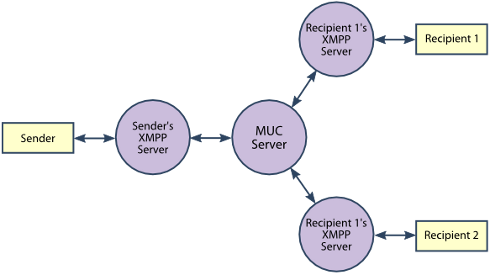
\includegraphics[scale=0.8]{images/MUC.png}   
		\caption[MUC]{MUC System Architecture}     
		\label{img:muc-architecture}                    
		\end{figure}

\emph{Group Chat Services}
\newline
Group chat is provided as a service, usually alongside a regular XMPP server. The group chat service has its own domain; for example, the jabber.org server runs a group chat service at conference.jabber.org. Each room on the group chat service gets its own address, which looks just like a user’s JID. Rooms can have access controls, moderators, administrators, and even automatic logging and archival of the group’s communications.

\emph{Entering and Leaving a Room}
\newline
Before making any changes in a chat room a user have to enter the room. This is also often referred to as joining the room. After a user done, he leaves the room. Because this mirrors the concept of a user coming and going on and offline, the multi-user chat designers decided to model this part of the protocol with <presence> stanzas. Users can join a group chat room by sending available presence to the room, along with a note that they understand the multi-user chat protocol. Sending presence directly to a JID instead of to the user’s server is called directed presence. Similarly, to leave, unavailable presence is sent to the room. Sending presence stanzas directly to a JID instead of to the user’s server is called sending directed presence.

If Mark wants to join the group chat room with the Temperature sensor, they will both need to send directed presence to their desired identity in the room temperature@chat.sensor.lit. Their stanzas are shown in the Listing~\ref{code:stanzas_muc}:
\begin{lstlisting}[label=code:stanzas_muc,caption=Stanzas Format for MUC]
<presence to="temperature@chat.sensor.lit/sensor"
          from="sensor@example.lit/sensor">
    <x xmlns="http://jabber.org/protocol/muc"/>
</presence>
\end{lstlisting}

Once they have joined the room, the group chat service will broadcast all the other participants' presence statuses to them. After all the other participants’ presence stanzas are sent, the server concludes the presence broadcast by sending the arriving participant’s presence to everyone, including the new arrival. Thus, when a new participant sees their own presence broadcast back to them, they know they have fully joined the room.

The room sends the affiliations and roles of each participant along with their presence. Sensor's own presence broadcast also includes a status code of 110, which signals that this presence refers to the sensor itself. Just as with presence updates from sensor's roster, sensor will also receive presence updates from the room as people leave and new people join on the listing~\ref{code:muc_affiliation}.
\begin{lstlisting}[label=code:muc_affiliation,caption=Server Presence Notification]
<presence to="sensor@example.lit/sensor"
          from="temperature@chat.sensor.lit/sensor">
  <x xmlns="http://jabber.org/protocol/muc">
      <item affiliation="member" role="participant"/>
      <status code="110"/>
  </x>
</presence>
\end{lstlisting}

\textbf{Creating Rooms}
\newline
Creating rooms is accomplished in the same manner as joining a room. Assuming the service allows the user to create new rooms, sending directed presence to the desired room JID of the new room will cause the room to be created and the user to be set as the room’s owner. On the Listing~\ref{code:room_creation}, sensor creates a new room for the News feed.

	\begin{lstlisting}[label=code:room_creation,caption=MUC Room Creation]
<presence to="chatter@chat.news.lit/sensor"
          from="sensor@news.lit/drawing_room">
    <x xmlns="http://jabber.org/protocol/muc"/>
</presence>
	\end{lstlisting}

The chat.news.lit service responds with the presence broadcast for the room’s new and only occupant(Listing~\ref{code:server_respond}).

	\begin{lstlisting}[label=code:server_respond,caption=Server Respond to Room Creation]
<presence to="sensor@news.lit/drawing_room"
          from="chatter@chat.news.lit/sensor">
    <x xmlns="http://jabber.org/protocol/muc">
        <item affiliation="owner" role="moderator"/>
        <status code="110"/>
        <status code="20"/>
    </x>
</presence>
		\end{lstlisting}

Sensor has the owner affiliation and the moderator role. These attributes give the sensor special permissions within the room. The 110 status code is sent, just as it was before, and a new status code of 201 is sent, it signals that a new room has been created. More comprehensive information about roles, affiliations, erros and etc can be found in documentation \cite{XMPPbook}.

\subsection{XEP-0060: Publish-Subscribe}
Publish-subscribe XMPP extension\footnote{XEP-0060: Publish-Subscribe, \url{http://xmpp.org/extensions/xep-0060.html}} provides a framework for a wide variety of applications, including news feeds, content syndication, extended presence, geolocation, trading systems, workflow systems, and any other application that requires event notifications (image~\ref{img:basic-pubsub}.

\begin{figure}[!ht]
    \centering
    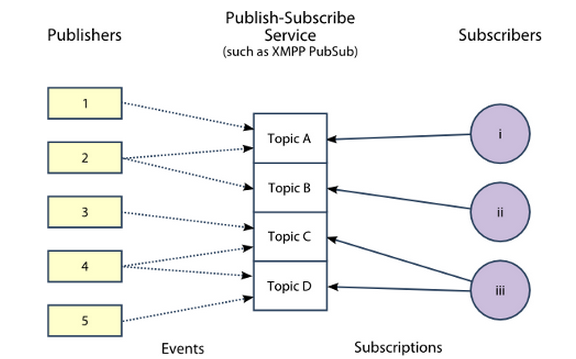
\includegraphics[scale=0.5]{images/XEP0049.png}   
    \caption[General Event Subscription]{General Event Subscription}  
    \label{img:basic-pubsub}                    
\end{figure}

There is a channel of communication, subscribers who are interested in data sent on that channel, and publishers who can send data across the channel. The first thing an application must do for a presenter is to create a channel to publish information. In XMPP pubsub these channels are called \emph{nodes}. The protocol enables XMPP entities to create nodes (services) at a pubsub service and publish information at those nodes; an event notification (with or without payload) is then broadcasted to all entities that have subscribed to the node. Pubsub therefore adheres to the classic Observer design pattern.

	\textbf{Creating a Node}
	\newline
	A pubsub node is created by sending an IQ-set stanza to the pubsub service, as shown in the listing~\ref{code:node_creation}, where User1 creates node ``sensor\_data'' within ``pubsub.sensor1.lit'' XMPP host server.
		\begin{lstlisting}[label=code:node_creation,caption=PubSub Node Creation]
	<iq to="pubsub.sensor1.lit"
	    from="user_1@sensor1.lit/sensor_registry"
	    type="set"
	    id="create1">
	  <pubsub xmlns="http://jabber.org/protocol/pubsub">
	      <create node="sensor_data"/>
	  </pubsub>
	</iq>
		\end{lstlisting}
	Most actions on pubsub nodes will look very similar to this one, the difference between MUC and PubSub stanzas is the <pubsub> element. Pubsub nodes and their configuration are necessary and useful, but they don't do much by themselves. The real value of pubsub nodes is in the events that are published to them and broadcast to subscribers. Anything can be included in a pubsub event. The pubsub service doesn’t know or care what is inside the event; it simply broadcasts this data to a node’s subscribers.

\textbf{Retrieving Item}
\newline
User2 just subscribed to user1's sensor\_data node, and has missed his earlier event broadcasts.  User1 configured his node to persist items and anyone can query his node for the most recently published items. In listing~\ref{code:last-5-items}, user2 requests the last five items by sending an IQ-get stanza to the node with the <items>:
\begin{lstlisting}[label=code:last-5-items,caption=PubSub: requesting last 5 items from history]
<iq from="user2@longbourn.lit/outside"
    to="pubsub.sensor1.lit"
    type="get"
    id="items1">
  <pubsub xmlns="http://jabber.org/protocol/pubsub">
    <items node="sensor_data" max_items="5"/>
  </pubsub>
</iq>
\end{lstlisting}
The <items> element contains a node attribute just like the other actions. User2 has also set the max\_items attribute to 5 because he is only interested in the recent history. If he had omitted max\_items, the server would interpret it as a request to send all the historical data it has been configured to keep. If he had set max\_items to 500, which is much larger than the configured maximum for the node, the server would have sent as many as were available.

\textbf{PubSub Data Flow}
\newline
Figure 5.8 shows the process flow of how and when a client can subscribe/retrieve data from a publisher of service through the XMPP PubSub approach. The first thing the DataSource 1 and 2 must do for a would-be presenter is to create a channel for them to publish data - nodes. Once a node is created and configured, Publishers can start send data. Once these events are published, pubsub takes over and makes sure that they get delivered to the subscribed users. In case Publishers want to get a list of their subscribers, it can be retrieved from the pubsub node so that it can present this data to them. If Publisher will become offline its <presence> will be changed automatically to ``unavailable'' and next time, becoming online and sending new data, all subscribers will receive this information immediately.
    \begin{figure}[!ht]
    \centering
    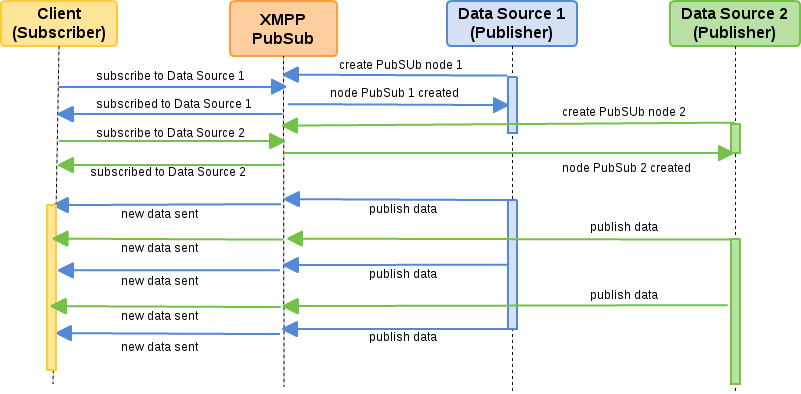
\includegraphics[scale=0.6]{images/PubSub.png}   
    \caption[Service PubSub]{Service PubSub}
    \label{img:pub_sub}                           
    \end{figure}
	    
 \subsection{PubSub vs MUC}
	\textbf{Pubsub Advantages}
	\newline
	Publish-subscribe is a very generic system, used by many different kinds of applications. The XMPP pubsub extension is similarly generic and is usable for a wide variety of purposes. It assumes nothing about the subscribers; they may be human, or they may be machines. Pubsub nodes, unlike multi-user chat rooms, are arranged in a tree-based hierarchy. This shape is often a more close match to a given problem domain. One of the benefits of the tree shape is that entities can subscribe to non-leaf nodes of the tree, and events published below that node can also be received. Events can be published as notifications or as full payloads, and the subscriber can choose which is most appropriate. Retrieval of the publishing history is built in and fairly fine grained. The subscriber has more fine grained control over the delivery destination. 

	\textbf{Pubsub Disadvantages}
	\newline
	Pubsub, by being so generic, is not optimized for specialized cases. The pubsub extension is not nearly as old or as widely implemented as MUC, and the support for features in both clients and servers varies in quality and depth. Unlike MUC, it is not yet clear what the most used features are, so one must shop around a bit when an advanced feature is needed. There is no special handling of presence built in. There are a few proposed extensions to pubsub that may change this. For example, it would sometimes be useful to limit delivery to available resources only. Tooling for pubsub node creation and configuration is lacking. MUC room creation and configuration is built in to most XMPP clients already. Pubsub has not built-in mechanism for subscribers to interact or find each other. 

	\textbf{Multi-User Chat Advantages}
	\newline
	Presence handling is built in to MUC at a low level. Presence is used to signal joining and leaving of room, and presence changes can also be shared with occupants of the room. MUC is optimized for chat-related use cases and builds on the decades of experience of previous chat systems, especially IRC. All the common moderation and administration features necessary in a collaborative environment are supported - kicking, banning, and various privilege levels. MUC already has many implementations, both of clients and of servers. It is one of the oldest XMPP extensions, and as such, is quite mature and robust. Occupants in MUC rooms can interact with each other, and MUC allows for multiple levels of anonymity to be used as well as private communication.

	\textbf{Multi-User Chat Disadvantages}
	\newline
	Groups of people chatting is the bread and butter of MUC, and MUC is highly optimized for this use case. For example, most MUC servers will automatically send conversation history to every new occupant and generate human-readable messages for most administrative actions. It's possible, and common, to have bots as room occupants, but the experience is designed for human consumption. There is no way to organize chat rooms except as a flat hierarchy, and there is no way to share configurations or participation across collections of rooms. The one exception to this is that most servers have a default configuration that is applied to all rooms on the server. All of these extra human-focused features and administration capabilities make implementation more difficult. Unlike pubsub, MUC implementations have a lot of edge cases in order to be user friendly and robust.


\subsection{XEP-0049: Private XML Storage}
	Private XML Storage\footnote{XEP0049 specification,\url{http://xmpp.org/extensions/xep-0049.html}} is a Jabber extension, allowing a client to store any arbitrary XML on the XMPP server by sending an <iq/> stanza of type ``set'' to the server with a <query/> child scoped by the ``jabber:iq:private'' namespace. The <query/> element may contain any arbitrary XML fragment as long as the root element of that fragment is scoped by its own namespace. The data can then be retrieved by sending an <iq/> stanza of type ``get'' with a <query/> child scoped by the ``jabber:iq:private'' namespace, which in turn contains a child element scoped by the namespace used for storage of that fragment. Using this method, Jabber entities can store private data on the server and retrieve it whenever necessary. The data stored might be anything, as long as it is valid XML. One typical usage for this namespace is the server-side storage of client-specific preferences. All available methods are displayed in table~\ref{img:xep49-methods}.
	
	\begin{figure}[!ht]
		\centering
		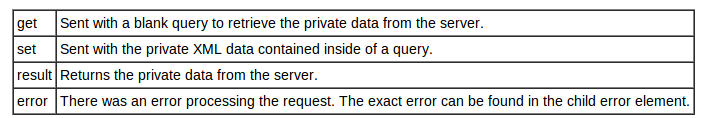
\includegraphics[scale=0.9]{images/xep0049Queries.png}   
		\caption[ Description of Acceptable Methods]{Description of Acceptable Methods}
		\label{img:xep49-methods}
		\end{figure}
	\subsubsection{Elements}
	The root element of Private XML Storage namespace is query. At least one child element with a proper namespace must be included; otherwise the server must respond with a ``Not Acceptable'' error. A client must not query for more than one namespace in a single IQ get request. However, an IQ set or result may contain multiple elements qualified by the same namespace. Examples of saving and loading data are shown on listing~\ref{code:client_save} and ~\ref{code:client_load}.

    \begin{lstlisting}[label=code:client_save,caption=Client Stores Private Data]
		CLIENT:
		<iq type="set" id="1001">
		  <query xmlns="jabber:iq:private">
		    <exodus xmlns="exodus:prefs">
		      <defaultnick>Alice</defaultnick>
		    </exodus>
		  </query>
		</iq>

		SERVER:
		<iq type="result"
		    from="alice@likepro.co/"
		    to="alice@likepro.co/"
		    id="1001"/>
    \end{lstlisting}

     \begin{lstlisting}[label=code:client_load,caption=Client Retrieves Private Data]
		CLIENT:
		<iq type="get" id="1001">
		  <query xmlns="jabber:iq:private">
		    <exodus xmlns="exodus:prefs"/>
		  </query>
		</iq>

		SERVER:
		<iq type="result"
		    from="alice@likepro.co/"
		    to="alice@likepro.co/"
		    id="1001">
		  <query xmlns="jabber:iq:private">
		    <exodus xmlns="exodus:prefs">
		      <defaultnick>Alice</defaultnick>
		    </exodus>
		  </query>
		</iq>
    \end{lstlisting}

    The message format described above can be made by using two main functions: save(for saving data on the XMPP server) and load(to retrieve saved data from the XMPP server), as shown on the Listing~\ref{save_load_ns}:
	\begin{lstlisting}[label=save_load_ns,caption=Snippet of Save/Load preferences to a private namespace]
	      	save: function (property) {
	            xmpp.connection.private.set(property, property + ":ns", user[property], function (data) {
	                    console.log(property + " saved: ", data);
	                },
	                console.log);
	        },
	        load: function (property) {
	            xmpp.connection.private.get(property, property + ":ns", function (data) {
	                    user[property] = data != undefined ? data : [];
	                    if (property == 'subscriptions') {
	                        for (var i = 0; i < user.subscriptions.length; i++) {
	                            xmpp.subscribe(user.subscriptions[i]);
	                        }
	                    }
	                    $rootScope.$apply();
	                },
	        }
	\end{lstlisting}


%%%%%%%%%%%%%%%%%%%%%%%%%%%%%%%%%%%%%%%%%EVALUATION%%%%%%%%%%%%%%%%%%%%%%%%%%%%%%%%%%%%%%%%%%%%%%%%%%%%%%%%%%%%%%%%%%%%
\section{Evaluation}
Evaluation are done as a proof of concept by demonstrating a scenario of distributed XMPP-driven web site accessing data from a hardware and software sensors. Where as software sensor was taken a bot, which periodically sends some IT news in a text format. And as a hardware sensor was used a temperature sensor from university. To the prototype was given a name: SensDash(Sensor Dashboard). Temperature sensor was provided as a testing environment in scope of ACDSee project, together with TU Dresden, BTU Cottbus - Senftenberg and RWTH Aachen University. It locates in the room INF3084, Faculty of Information Technology, Chair of Computer Science. The sensor part represents a class of low-cost, high-performance sensors. It is implemented using a commercially available Raspberry Pi single-board computer with an affiliated USB thermometer and automatic WLAN and XMPP connections to a sensor MUC room established at boot time. Everything concerning sensor are installed on Mobilis server. According to the system architecture on the Figure 5.10, everything concerning sensor data are assumed implemented on a DataHub. Which has pre-installed XMPP server supporting MUC rooms, each carry a description field which qualifies them as sensor MUC rooms. The temperature sensor itself is a Data Source 1 and Data Source 2 respectively is a software sensor  presented on the Figure 5.10.

The temperature sensor available from a MUC room: xmpp://inf3084@conference.mobilis-dev.inf.tu-dresden.de and has the next JSON description(Listing~\ref{json_sensor_1}):
	\begin{lstlisting}[label=json_sensor_1,caption=JSON Description Format]
{
    "sensormuc": {
        "type": "AMBIENT_TEMPERATURE",
        "format": "short",
        "location": {
            "countryCode": "DE",
            "cityName": "Cottbus",
            "latitude": 51.076834,
            "longitude": 13.772586
        }
    }
}
	\end{lstlisting}
     \begin{figure}[H]
        \centering
        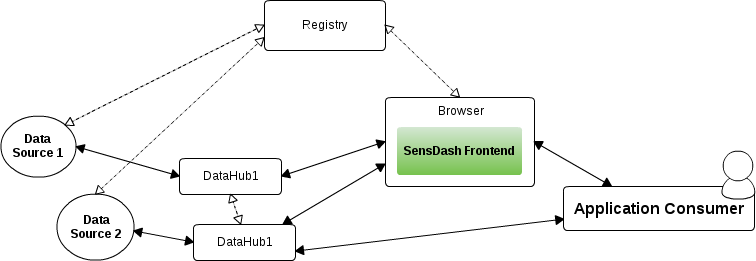
\includegraphics[scale=0.6]{images/UseCaseScheme1.png}   
        \caption[Use Case System Architecture Scheme]{System Architecture Scheme}                         
        \end{figure}
Firstly it has to be registered in the Sensor Registry with an unique id and fulfill the attributes defined in JSON Registry standard accordingly. Since in scope of Master Thesis neither in scope of ACDSee project not included to implement automative Registry, where sensor have to be registered, metadata describing temperature sensor was added manually. The full example of metadata existed in Registry can be found in Appendix A, and the Listing~\ref{sensor_registry} below presents only main charactristics, defined as attribute:
	\begin{lstlisting}[label=sensor_registry,caption=JSON Description Format]
[
    {
            "id": "30",
            "title": "Ambient Temperature INF3084",
            "availability": true,
            "description": "DSE students receive an opportunity to get current outdoor temperature in Dresden Momsenstr.20. This sensor provides temperature updates with 5-second frequency and represents a class of low-cost, high-performance sensors. It is implemented using a commercially available Raspberry Pi single-board computer with an affiliated USB thermometer and automatic WLAN and XMPP connections to a sensor MUC room established at boot time.",
            "sla": "Sensor resolution is 0.5 C, measurements taken every 5 seconds. Uptime 95% from 6:00 till 22:00.",
            "sla_last_update":"1395005996",
            "access": "private",
            "provider_name": "Provider TU Dresden",
            "location": "Dresden",            
            "type": "chart",
            "end_points": [
                {
                    "type": "muc",
                    "name": "xmpp://inf3084@conference.mobilis-dev.inf.tu-dresden.de",
                    "pwd": null
                },
                {
                    "type": "muc",
                    "name": "xmpp://inf3086@conference.mobilis-dev.inf.tu-dresden.de",
                    "pwd": null
                }

            ]
    }
]
	\end{lstlisting}
Demonstration of activity scenario was made by using 3d party user which is application consumer developer. His name Max and he has to create specific mobile application. A sa result, firstly he needs to define which sensors to use and how to retrieve an info from it. 
\subsection{Use Case Scenario}
\label{section:use-case-scenario}

\textbf{Step 1:} In order to find necessary sensor, explore description and data provided by it, Max has to sign in into the SensDash by using peronal JID and password, received from an dministrator of a SensDash(Figure 5.11).
\begin{figure}[!ht]
\centering
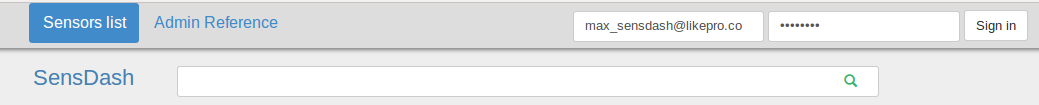
\includegraphics[scale=0.6]{Screenshots/signIn.png}   
\caption[Log in to the SensDash]{Log in to the SensDash}                         
\end{figure}

\textbf{Step 2:} After successfully passing authorisation, Max can start searching necessary sensors. By using search field, he can enter the one of the key word which is clearly define purpose or type of a sensor, and immediately list of sensors will be sorted based on his search input. To get more detailed information about sensor he clicks on the field of sensor. In a new popup window(Figure 5.12), and if to be more precise, it is a new tool, called modal. In the appeared modal, user can get a detailed description about sensor, e.g. : SLA, location, provider, preview, development details such as end-points quantity, end-point configuration, administrator name and of course more sophisticated description. This information gives an overview of what type of data provided by data source. 
\begin{figure}[!ht]
\centering
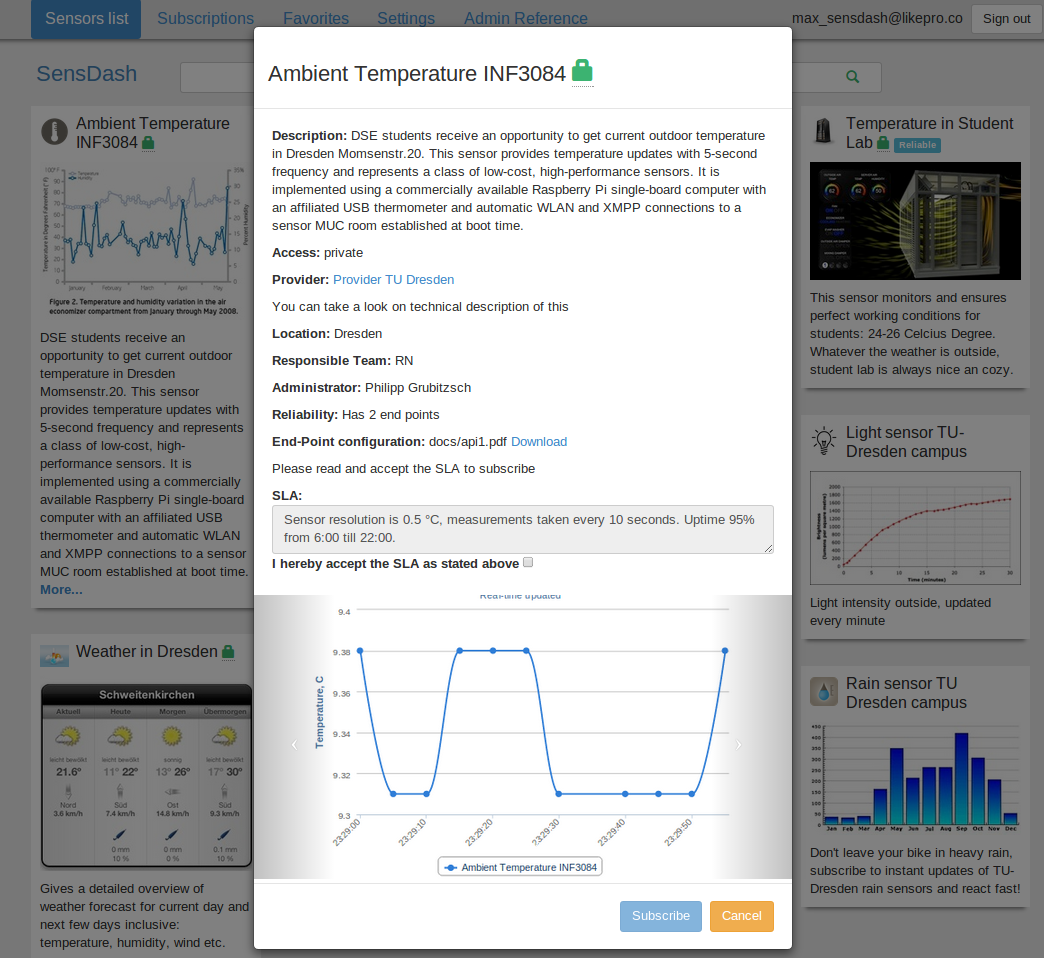
\includegraphics[scale=0.6]{Screenshots/UseCaseWelcome.png}   
\caption[Personal Modal of a Sensor]{Personal Modal of a Sensor}                         
\end{figure}
 
 In case of ambient temperature INF3084, Max can explore predefined preview, which consists graph of provided temperature, data values and it's frequency, security level and relialability. In case of software sensor it can be sample of news feed, provided by sensor. 

\begin{figure}[!ht]
\centering
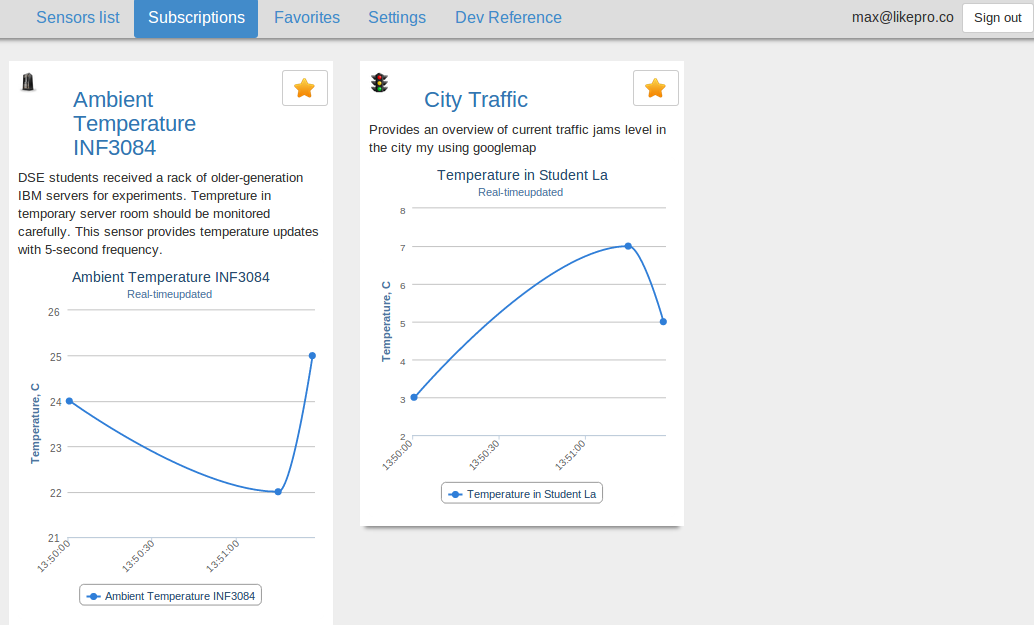
\includegraphics[scale=0.6]{Screenshots/UseCaseScreenshot4.png}   
\caption[Personal Subscribed Sensor]{Subscriptions list}                         
\end{figure}
\textbf{Step 3:} Since the ambient temperature sensor is a private sensor, Max has to accept SLA before getting a real-time data from it. In contrast to temperature sensor, a software sensor - IT news feed has a public access, thus, Max doesn't need to accept any SLA in order to see real-time data provided by this sensor. The common rule, which is applied to every sensor independently from its access type(public or private) is to subscribe to it. In such a way, all sensors, to which Max has subscribed will appear in the next tab called "Subscriptions". And as soon as new data become available SensDash retrieve it in this (Figure 5.13). Also, by using Subscriptions Tab and icon "star" in a right corner, become possible to add subscribed sensor to the Favorites. After clicking on the icon of favorites, sensor information will appear in a list of favorites in Favorites Tab.

\textbf{Step 4:} To get info about personal account Max have to use Settings Tab. Where exists personal profile settings(Figure 5.14). 
\begin{figure}[!ht]
\centering
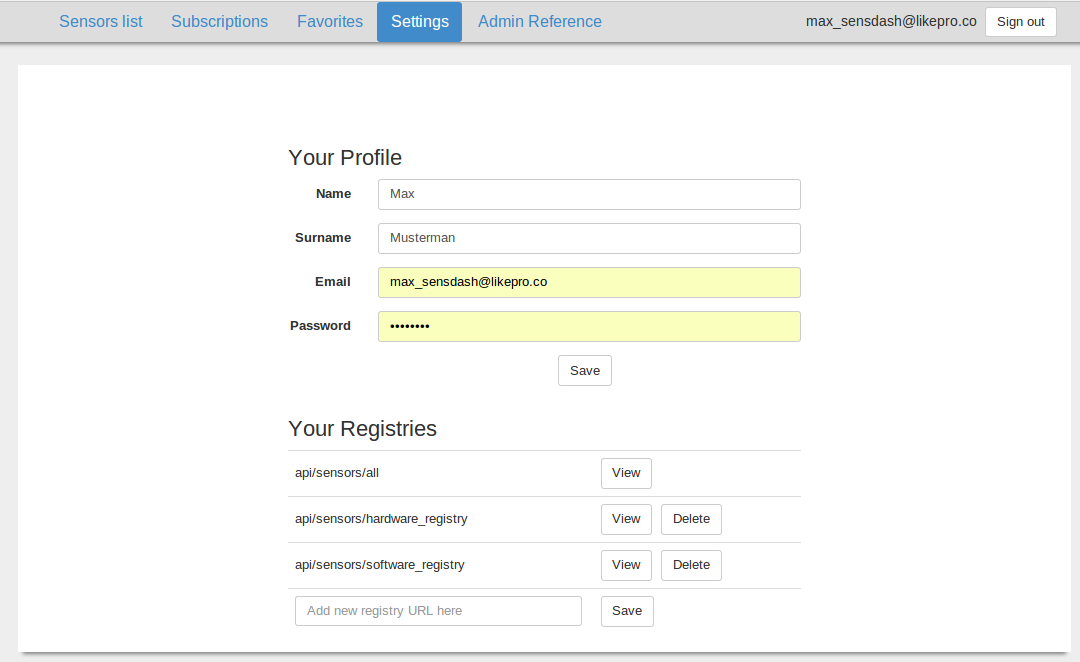
\includegraphics[scale=0.6]{Screenshots/UseCaseScreenshot6.png}   
\caption[Settings Tab]{Settings Tab}                         
\end{figure}

\textbf{Step 5:} As a developer, Max might be interested in technical details of sensor data retieval process, e.g. API references, end-point configuration, sensor data format, interface and system architecture in order to interconnect with backend directly. So Max has to go to the Admin References Tab(Figure 5.15), where he can find all available implementation detailes of a frontend itself, protocol and its extensions realization and system architecture. 
\begin{figure}[!ht]
\centering
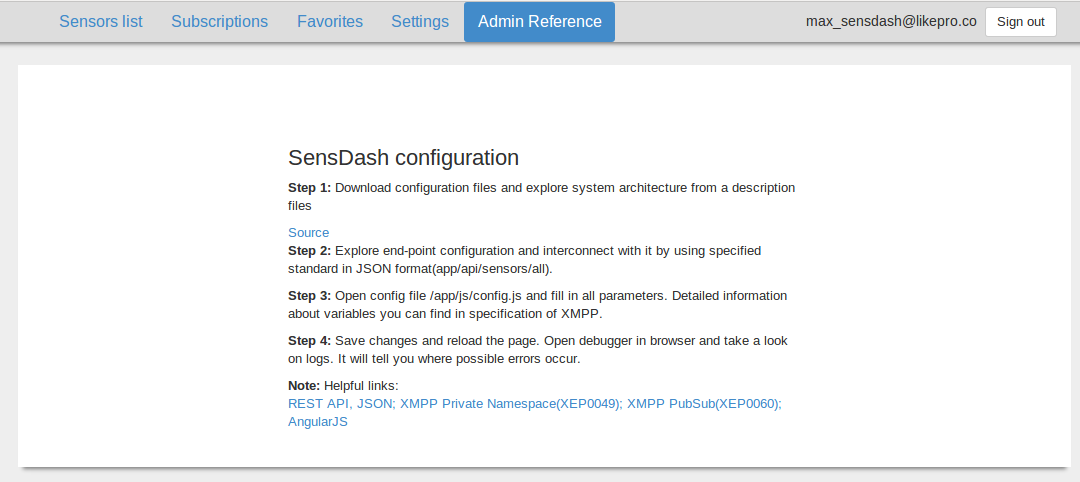
\includegraphics[scale=0.6]{Screenshots/UseCaseReferences.png}   
\caption[Administrator Tab]{Administrator Tab}                         
\end{figure}

\subsection{SensDash Implementation}
After real example of SensDash usage was described in the previous section, needs to be clarified the concept overflow together with used and implemented XMPP extensions.

\textbf{Log In}to the system can be possible only with valid JID and password, which have to be registered within any possible XMPP server. Since XMPP network structured very similar to DNS, doens't metter where registered JID. The only one important thing is to know which XMPP server carry on MUC room. Firstly, user credentials validated by input type on frontend side and only than sended to the backend. Once XMPP server authorize the user, JID and password are saved in a browser by using cookies. So the next time when the user will open abrowser URL of a SensDash, cookies will automatically log him/her into the system. 

\textbf{Preferences Saving} are done by using XEP0049 and stored on the XMPP server. When a user sign in to the system first time, application logic creates fully empty account with no subscriptions and favorites. Once a user subscribes to any resource, this resource automatically appear on Subscriptions Tab and added to the subscriptions map. The same for favorites and Favorite Tab, but favorites, due to simple structure are saved in a simple favorites array. It means that system has saved this preferences on XMPP server by using one of the extension called XEP0049, based on private space for every JID without interconnection with backend. Next time when user will log in to the system, all saved subscriptions and favorites will be loaded in the meanwhile and appear in corresponding tabs. An example subscriptions map and favorites array for Max are presented in Appendix B.

\subsubsection{Functional characteristic of a sensor}
In the section 4.4 was clarified 3 main characteristics which acquire sensor based on a system architecture. Since realization of a Data Hub fully rely on a backend, but in proposed evaluation was used XMPP server, become possible to differentiate security, reliability and performance level based only on a server configuration. Where every end-point is a MUC chat room(Figure 5.16). 
\begin{figure}[!ht]
\centering
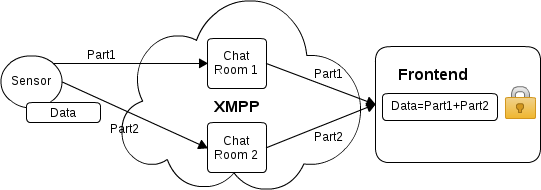
\includegraphics[scale=0.6]{images/security.png}   
\caption[Security]{Data secure transfer using Chat Rooms}                         
\end{figure}
Application logic calculate automatically number of available end-points for every sensor, based on Registry info and shows it on the main page as shown above on the Figure 5.17. The rules of how was calculated the security level or reliability are described in the Section 4.4, Subsection "Sensor Functional Characteristics"(Appendix C).
\newline
\begin{figure}[!ht]
\centering
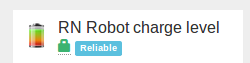
\includegraphics[scale=1.0]{Screenshots/Icons.png}   
\caption[GUI identification of security and reliability level]{GUI identification of security and reliability level}    
\end{figure}

\textbf{Search Bar} is made by using only frontend, as one of the feature of the AngularJS. It makes sorting of an graphical object through the all existed titles of a data source. It is fast and very straightforward in use. 

\textbf{Data Streaming} is the point where Data Hub as a part of a backend come into a picture. All data streaming works through XMPP extensions called XEP0049(MUC) or XEP0045(MUC). In presented example with ambient temprature in INF3084 was used MUC for retrieving real-time data throug the BOSH. Since generic frontend supposed to support all possible approaches, it also provides realization for PubSub(XEP0060). By using Strophe.js as a client-side web-based library was made refactoring according to skeleton defined by AngularJS. 
\newline
The SensDash logic builded on top of AngularJS skeleton(Appendix D). By using two-way data binding, aggregation and presentation of a sensor metadatadata was done by using factory pattern. Together with creation of a sensor entity as a graphical object, all handlers, functionality and interconnection protocol also created for every object accrodnigly, based on abstract methods. Such a general manipulation of objects makes possible to loosely couple code and object. All sensors metadata will be automatically parsed from Sensor Registry and presented on a SensDash always in the same way. Everything done in runtime, such that if a new sensor registers itself in Registry it will appear as soon as user reload the page. 

\section{Summary}
This chapter presents details of implementation of the generic frontend concept and proposes first working prototype, which is shown by using convincing scenario in the evaluation section 5.5. 

At the begining of a chapter, choosen tools and development environment were discovered and presented: jQuery, HTML5, CSS as a programming languages, AngularJS together with Bootstrap to interconnect application logic with XMPP interface standard and Strophe.js was picked to implement the XMPP mechanism and it's extensions. Web API was defined and afterwards used to retrieve from the Registry all available sensors by sending direct HTTP GET request to the Registry. Authentification and data streaming handling through the XMPP server was made by using XMPP BOSH standard and XEP0049, XEP0045 extensions, based on Strophe.js. In order to connect, disconnet, authorize, save, load, initiate connection through the XMPP interface all these methods and functions was refactored as skeleton, based on AngularJS directives and syntax. 

Was presented the convinsing scenario based on ambient temperature sensor from room INF3084(hardware sensor) and IT news Feed(software sensor) and consumer application developer's requirements.

All used technologies, protocols, libraries and methodologies was gathered together in order to realize working prototype. A summary overview of all implemented above components and tools are shown on the Figure 5.18.
\begin{figure}[H]
\centering
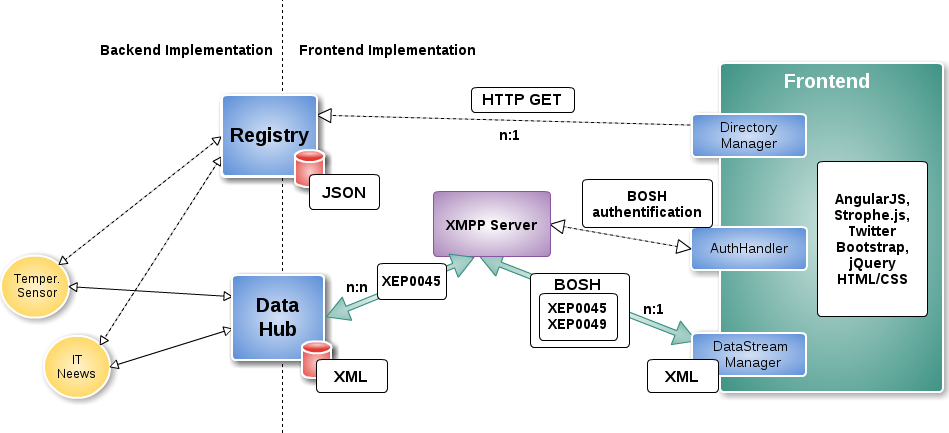
\includegraphics[scale=0.5]{images/ch5Summary.png}   
\caption[Implementation Architecture]{Integrated Implementation Architecture}                         
\end{figure}

